\documentclass[sigchi]{acmart}

\usepackage[utf8]{inputenc}
\usepackage[english]{babel}
\usepackage{booktabs} 	% For formal tables
\usepackage{listings}   % Writing code in latex document
\usepackage{hyperref} 	% For hyperlinks

\hypersetup{
  colorlinks=true,
  linkcolor=blue,
  filecolor=blue,      
  urlcolor=blue,
}

\graphicspath{{images/}}

\begin{document}
\title{Proposal}
\subtitle{Medical Imaging Diagnosis Assertiveness Alignment}

\author{Francisco Maria Calisto}
\orcid{0000-0001-8179-7872}
\affiliation{%
  \institution{Instituto Superior T\'{e}cnico}
  \city{Lisboa}
  \state{Portugal}
  \postcode{1049-001}
}
\email{francisco.calisto@tecnico.ulisboa.pt}

% The default list of authors is too long for headers.
\renewcommand{\shortauthors}{Calisto}


\begin{abstract}

This report provides the analysis and debate of a \textit{Medical Imaging Diagnosis Assertiveness Alignment} proposal.
In context of this document, it was created for the \hyperlink{https://fenix.tecnico.ulisboa.pt/disciplinas/TASE4/2019-2020/2-semestre}{Advanced Topics in Entertainment Systems} course of the \hyperlink{https://fenix.tecnico.ulisboa.pt/cursos/deic/curriculo}{Computer Science and Engineering Doctoral Program} at \hyperlink{https://tecnico.ulisboa.pt/en/}{IST} of \hyperlink{https://www.ulisboa.pt/}{ULisboa} - \hyperlink{https://www.portugal.gov.pt/en/}{Portugal} (\hyperlink{https://europa.eu}{EU}).

This document describes a proposal development and concept of a study to understand how the level of assertiveness, displayed by an AI assistant agent, will impact the radiologists' decision-making process during breast cancer diagnosis.
We will develop a proof-of-concept prototype, a medical imaging assistant, with two scenarios of the assistant behaviour:
(1) one scenario for an Assertive assistant; and
(2) a second scenario for a Non-Assertive assistant.
We will conduct a 2x4, between subjects experiment (n = 4 expected), in which Assertive and Non-Assertive subjects will be matched with the four categories of radiologists' professional experience, {\it i.e.}, Interns, Juniors, Middles and Seniors.
From a latter study, we will extract the rates of False-Positives and False-Negatives to understand patterns of critical behaviour among the four categories of professional experience.
In the end, we will propose several strategies that we expect to promote the unbiased behaviour per each professional experience, improving the False-Positives and False-Negatives rates during diagnostic.

\end{abstract}

\begin{teaserfigure}
\includegraphics[width=\textwidth]{teaser}
\end{teaserfigure}


\maketitle

\section{Introduction}
\label{sec:sec001}

The \textit{proceedings} are the records of a conference.\footnote{This
  is a footnote}  ACM seeks
to give these conference by-products a uniform, high-quality
appearance.  To do this, ACM has some rigid requirements for the
format of the proceedings documents: there is a specified format
(balanced double columns), a specified set of fonts (Arial or
Helvetica and Times Roman) in certain specified sizes, a specified
live area, centered on the page, specified size of margins, specified
column width and gutter size.

\section{The Body of The Paper}
\label{sec:sec002}
Typically, the body of a paper is organized into a hierarchical
structure, with numbered or unnumbered headings for sections,
subsections, sub-subsections, and even smaller sections.  The command
\texttt{{\char'134}section} that precedes this paragraph is part of
such a hierarchy.\footnote{This is a footnote.} \LaTeX\ handles the
numbering and placement of these headings for you, when you use the
appropriate heading commands around the titles of the headings.  If
you want a sub-subsection or smaller part to be unnumbered in your
output, simply append an asterisk to the command name.  Examples of
both numbered and unnumbered headings will appear throughout the
balance of this sample document.

Because the entire article is contained in the \textbf{document}
environment, you can indicate the start of a new paragraph with a
blank line in your input file; that is why this sentence forms a
separate paragraph.

\subsection{Type Changes and {\itshape Special} Characters}

We have already seen several typeface changes in this sample.  You can
indicate italicized words or phrases in your text with the command
\texttt{{\char'134}textit}; emboldening with the command
\texttt{{\char'134}textbf} and typewriter-style (for instance, for
computer code) with \texttt{{\char'134}texttt}.  But remember, you do
not have to indicate typestyle changes when such changes are part of
the \textit{structural} elements of your article; for instance, the
heading of this subsection will be in a sans serif\footnote{Another
  footnote here.  Let's make this a rather long one to see how it
  looks.} typeface, but that is handled by the document class file.
Take care with the use of\footnote{Another footnote.}  the
curly braces in typeface changes; they mark the beginning and end of
the text that is to be in the different typeface.

You can use whatever symbols, accented characters, or non-English
characters you need anywhere in your document; you can find a complete
list of what is available in the \textit{\LaTeX\ User's Guide}
\cite{Lamport:LaTeX}.

\subsection{Math Equations}
You may want to display math equations in three distinct styles:
inline, numbered or non-numbered display.  Each of
the three are discussed in the next sections.

\subsubsection{Inline (In-text) Equations}
A formula that appears in the running text is called an
inline or in-text formula.  It is produced by the
\textbf{math} environment, which can be
invoked with the usual \texttt{{\char'134}begin\,\ldots{\char'134}end}
construction or with the short form \texttt{\$\,\ldots\$}. You
can use any of the symbols and structures,
from $\alpha$ to $\omega$, available in
\LaTeX~\cite{Lamport:LaTeX}; this section will simply show a
few examples of in-text equations in context. Notice how
this equation:
\begin{math}
  \lim_{n\rightarrow \infty}x=0
\end{math},
set here in in-line math style, looks slightly different when
set in display style.  (See next section).

\subsubsection{Display Equations}
A numbered display equation---one set off by vertical space from the
text and centered horizontally---is produced by the \textbf{equation}
environment. An unnumbered display equation is produced by the
\textbf{displaymath} environment.

Again, in either environment, you can use any of the symbols
and structures available in \LaTeX\@; this section will just
give a couple of examples of display equations in context.
First, consider the equation, shown as an inline equation above:
\begin{equation}
  \lim_{n\rightarrow \infty}x=0
\end{equation}
Notice how it is formatted somewhat differently in
the \textbf{displaymath}
environment.  Now, we'll enter an unnumbered equation:
\begin{displaymath}
  \sum_{i=0}^{\infty} x + 1
\end{displaymath}
and follow it with another numbered equation:
\begin{equation}
  \sum_{i=0}^{\infty}x_i=\int_{0}^{\pi+2} f
\end{equation}
just to demonstrate \LaTeX's able handling of numbering.

\subsection{Citations}
Citations to articles~\cite{bowman:reasoning,
clark:pct, braams:babel, herlihy:methodology},
conference proceedings~\cite{clark:pct} or maybe
books \cite{Lamport:LaTeX, salas:calculus} listed
in the Bibliography section of your
article will occur throughout the text of your article.
You should use BibTeX to automatically produce this bibliography;
you simply need to insert one of several citation commands with
a key of the item cited in the proper location in
the \texttt{.tex} file~\cite{Lamport:LaTeX}.
The key is a short reference you invent to uniquely
identify each work; in this sample document, the key is
the first author's surname and a
word from the title.  This identifying key is included
with each item in the \texttt{.bib} file for your article.

The details of the construction of the \texttt{.bib} file
are beyond the scope of this sample document, but more
information can be found in the \textit{Author's Guide},
and exhaustive details in the \textit{\LaTeX\ User's
Guide} by Lamport~\shortcite{Lamport:LaTeX}.

This article shows only the plainest form
of the citation command, using \texttt{{\char'134}cite}.

Some examples.  A paginated journal article \cite{Abril07}, an enumerated
journal article \cite{Cohen07}, a reference to an entire issue \cite{JCohen96},
a monograph (whole book) \cite{Kosiur01}, a monograph/whole book in a series (see 2a in spec. document)
\cite{Harel79}, a divisible-book such as an anthology or compilation \cite{Editor00}
followed by the same example, however we only output the series if the volume number is given
\cite{Editor00a} (so Editor00a's series should NOT be present since it has no vol. no.),
a chapter in a divisible book \cite{Spector90}, a chapter in a divisible book
in a series \cite{Douglass98}, a multi-volume work as book \cite{Knuth97},
an article in a proceedings (of a conference, symposium, workshop for example)
(paginated proceedings article) \cite{Andler79}, a proceedings article
with all possible elements \cite{Smith10}, an example of an enumerated
proceedings article \cite{VanGundy07},
an informally published work \cite{Harel78}, a doctoral dissertation \cite{Clarkson85},
a master's thesis: \cite{anisi03}, an online document / world wide web
resource \cite{Thornburg01, Ablamowicz07, Poker06}, a video game (Case 1) \cite{Obama08} and (Case 2) \cite{Novak03}
and \cite{Lee05} and (Case 3) a patent \cite{JoeScientist001},
work accepted for publication \cite{rous08}, 'YYYYb'-test for prolific author
\cite{SaeediMEJ10} and \cite{SaeediJETC10}. Other cites might contain
'duplicate' DOI and URLs (some SIAM articles) \cite{Kirschmer:2010:AEI:1958016.1958018}.
Boris / Barbara Beeton: multi-volume works as books
\cite{MR781536} and \cite{MR781537}.

A couple of citations with DOIs: \cite{2004:ITE:1009386.1010128,
  Kirschmer:2010:AEI:1958016.1958018}.

Online citations: \cite{TUGInstmem, Thornburg01, CTANacmart}.


\subsection{Tables}
Because tables cannot be split across pages, the best
placement for them is typically the top of the page
nearest their initial cite.  To
ensure this proper ``floating'' placement of tables, use the
environment \textbf{table} to enclose the table's contents and
the table caption.  The contents of the table itself must go
in the \textbf{tabular} environment, to
be aligned properly in rows and columns, with the desired
horizontal and vertical rules.  Again, detailed instructions
on \textbf{tabular} material
are found in the \textit{\LaTeX\ User's Guide}.

Immediately following this sentence is the point at which
Table~\ref{tab:freq} is included in the input file; compare the
placement of the table here with the table in the printed
output of this document.

\begin{table}
  \caption{Frequency of Special Characters}
  \label{tab:freq}
  \begin{tabular}{ccl}
    \toprule
    Non-English or Math&Frequency&Comments\\
    \midrule
    \O & 1 in 1,000& For Swedish names\\
    $\pi$ & 1 in 5& Common in math\\
    \$ & 4 in 5 & Used in business\\
    $\Psi^2_1$ & 1 in 40,000& Unexplained usage\\
  \bottomrule
\end{tabular}
\end{table}

To set a wider table, which takes up the whole width of the page's
live area, use the environment \textbf{table*} to enclose the table's
contents and the table caption.  As with a single-column table, this
wide table will ``float'' to a location deemed more desirable.
Immediately following this sentence is the point at which
Table~\ref{tab:commands} is included in the input file; again, it is
instructive to compare the placement of the table here with the table
in the printed output of this document.


\begin{table*}
  \caption{Some Typical Commands}
  \label{tab:commands}
  \begin{tabular}{ccl}
    \toprule
    Command &A Number & Comments\\
    \midrule
    \texttt{{\char'134}author} & 100& Author \\
    \texttt{{\char'134}table}& 300 & For tables\\
    \texttt{{\char'134}table*}& 400& For wider tables\\
    \bottomrule
  \end{tabular}
\end{table*}
% end the environment with {table*}, NOTE not {table}!

It is strongly recommended to use the package booktabs~\cite{Fear05}
and follow its main principles of typography with respect to tables:
\begin{enumerate}
\item Never, ever use vertical rules.
\item Never use double rules.
\end{enumerate}
It is also a good idea not to overuse horizontal rules.


\subsection{Figures}

Like tables, figures cannot be split across pages; the best placement
for them is typically the top or the bottom of the page nearest their
initial cite.  To ensure this proper ``floating'' placement of
figures, use the environment \textbf{figure} to enclose the figure and
its caption.

This sample document contains examples of \texttt{.eps} files to be
displayable with \LaTeX.  If you work with pdf\LaTeX, use files in the
\texttt{.pdf} format.  Note that most modern \TeX\ systems will convert
\texttt{.eps} to \texttt{.pdf} for you on the fly.  More details on
each of these are found in the \textit{Author's Guide}.

\begin{figure}

\includegraphics{fly}
\caption{A sample black and white graphic.}
\end{figure}

\begin{figure}

\includegraphics[height=1in, width=1in]{fly}
\caption{A sample black and white graphic
that has been resized with the \texttt{includegraphics} command.}
\end{figure}


As was the case with tables, you may want a figure that spans two
columns.  To do this, and still to ensure proper ``floating''
placement of tables, use the environment \textbf{figure*} to enclose
the figure and its caption.  And don't forget to end the environment
with \textbf{figure*}, not \textbf{figure}!

\begin{figure*}
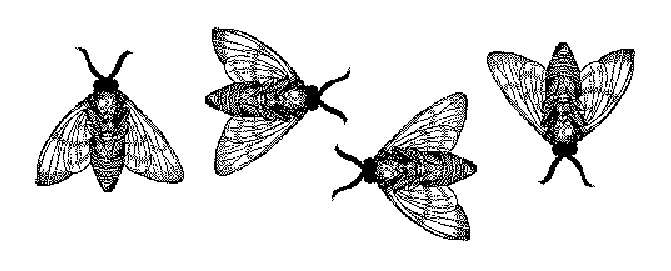
\includegraphics{flies}
\caption{A sample black and white graphic
that needs to span two columns of text.}
\end{figure*}


\begin{figure}
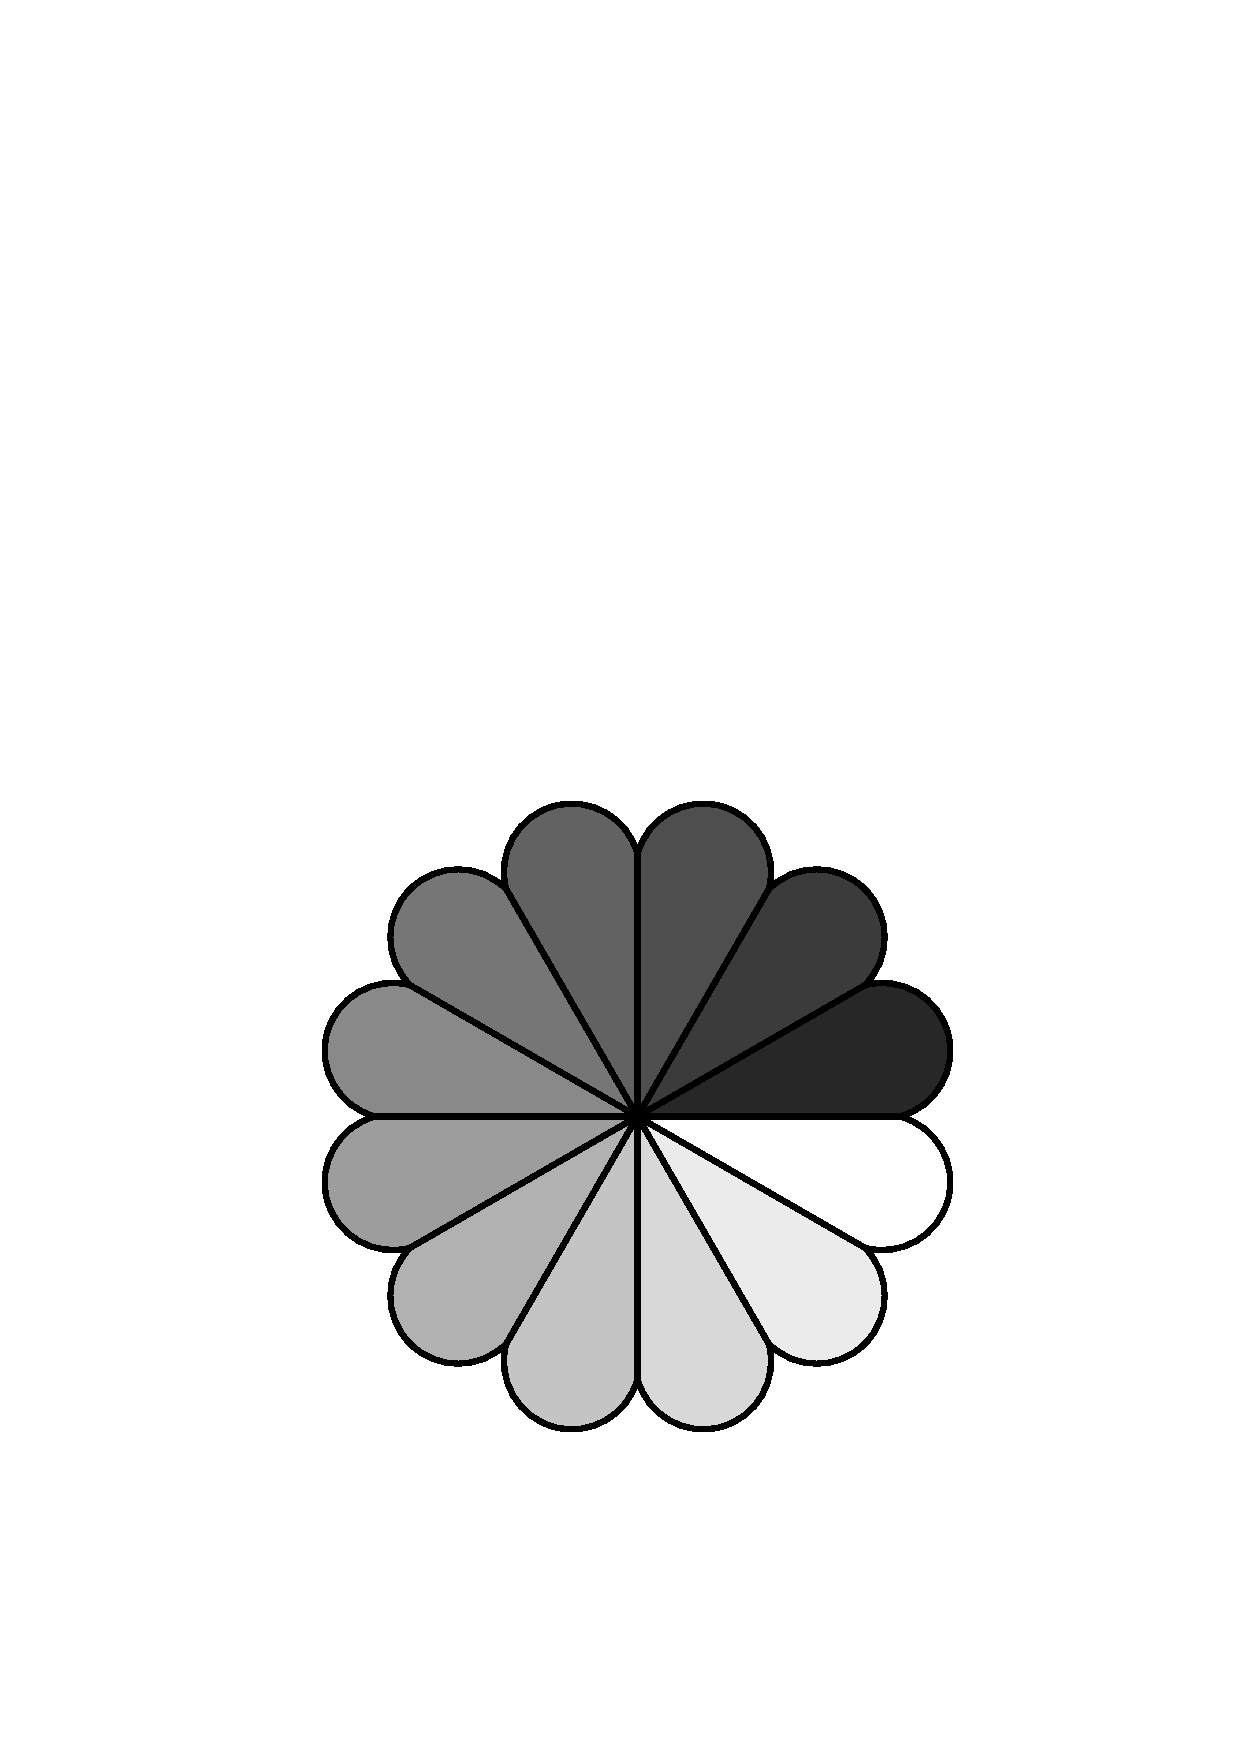
\includegraphics[height=1in, width=1in]{rosette}
\caption{A sample black and white graphic that has
been resized with the \texttt{includegraphics} command.}
\end{figure}

\subsection{Theorem-like Constructs}

Other common constructs that may occur in your article are the forms
for logical constructs like theorems, axioms, corollaries and proofs.
ACM uses two types of these constructs:  theorem-like and
definition-like.

Here is a theorem:
\begin{theorem}
  Let $f$ be continuous on $[a,b]$.  If $G$ is
  an antiderivative for $f$ on $[a,b]$, then
  \begin{displaymath}
    \int^b_af(t)\,dt = G(b) - G(a).
  \end{displaymath}
\end{theorem}

Here is a definition:
\begin{definition}
  If $z$ is irrational, then by $e^z$ we mean the
  unique number that has
  logarithm $z$:
  \begin{displaymath}
    \log e^z = z.
  \end{displaymath}
\end{definition}

The pre-defined theorem-like constructs are \textbf{theorem},
\textbf{conjecture}, \textbf{proposition}, \textbf{lemma} and
\textbf{corollary}.  The pre-defined de\-fi\-ni\-ti\-on-like constructs are
\textbf{example} and \textbf{definition}.  You can add your own
constructs using the \textsl{amsthm} interface~\cite{Amsthm15}.  The
styles used in the \verb|\theoremstyle| command are \textbf{acmplain}
and \textbf{acmdefinition}.

Another construct is \textbf{proof}, for example,

\begin{proof}
  Suppose on the contrary there exists a real number $L$ such that
  \begin{displaymath}
    \lim_{x\rightarrow\infty} \frac{f(x)}{g(x)} = L.
  \end{displaymath}
  Then
  \begin{displaymath}
    l=\lim_{x\rightarrow c} f(x)
    = \lim_{x\rightarrow c}
    \left[ g{x} \cdot \frac{f(x)}{g(x)} \right ]
    = \lim_{x\rightarrow c} g(x) \cdot \lim_{x\rightarrow c}
    \frac{f(x)}{g(x)} = 0\cdot L = 0,
  \end{displaymath}
  which contradicts our assumption that $l\neq 0$.
\end{proof}

\section{Clinical Design Keys}
\label{sec:sec003}

For this document, our goal is to propose a new study.
The study will describe how displaying different levels of assertiveness can influence clinician's responses to agents.
Moreover, we expect to understand the clinicians' behaviour during the decision-making process in a real-world setting.
In this section, we propose the analysis of a study where we devise a mixed-design prototype in which we will manipulate the level of assertiveness displayed by the assistant.

\subsection{Medical Procedures}
\label{sec:sec00301}

At this point, we will take impressions regarding the efficiency of clinicians, and their recommendations based on their experience for improvements of the patient examination.
In fact, several studies demonstrated~\cite{waite2017tired} that radiologist fatigue levels and performance are related to environmental factors such as number of FPs and FNs.
That said, we start analyzing the potential enhancement that an {\it AI-Assisted} diagnosis could take in the radiology room~\cite{chatelain2018evaluation, miglioretti2007radiologist}.

\subsection{Insights and Challenges}
\label{sec:sec00302}

Our observations and interviews will align with previous research on clinician-driven diagnostic {\it tasks}~\cite{Sultanum:2018:MTP:3173574.3173996}.
From the research insights we need to identify the following main challenges:
i) the heterogeneous visualization mode of a large number of images and file sizes;
ii) the annotation of medical images to support diagnosis and also 
how the introduction of the {\it AI techniques} can improve the classification ground-truth for; and
iii) when performing the classifications, the clinicians' gap in visualizing images from different modalities.

\subsection{Design Goals}
\label{sec:sec00303}

As demonstrative example of implementing a diagnostic assistant in the design of medical imaging systems, we need to propose several design goals.
The main design goals should be closely related to the research insights and the challenges of the previous section, namely:
(1) a collection of a ground truth annotations, namely masses in all imaging modalities and calcification lesions in MG (for both CC and MLO views);
(2) classification of the lesion severity using the BI-RADS~\cite{aghaei2018association};
(3) categorization of the breast tissues (dense vs non-dense);
(4) clinical co-variables, such as personal and family records; and
(5) visualizations for clinical summary which is crucial for a proper diagnosis and to perform patient follow-up.
The aforementioned design goals aim at promoting a reliable diagnosis information to clinical radiologists.
Pairwise with the related literature and our formative study, we found a number of current issues early addressed, including {\it medical imaging structure trade-offs}, {\it radiology room temporal awareness}, {\it image segmentation} and {\it radiologists system trust}.

\noindent
We fuse these five insights into three corresponding design goals, as follows:

%%%%%%%%%%%%%%%%%%%%%%%%%%%%%%%%%%%%%%%%%%%%%%%%%%
\begin{description}
\item[Medical Imaging Design (MID)] focusing on how to provide the best visualization strategy, given the heterogeneous information coming from the multi-modal sources of information;

\item[Control Result Design (CRD)] focusing on improving the physician's ability to {\it accept} or {\it reject} the {\it AI-Assisted} results;

\item[Based Explanation Design (BED)] focusing on increasing physicians understanding of how the AI techniques operate. By increasing understanding of how AI works, physicians can update their expectations of how well and in which situations the system is likely to work;
\end{description}
%%%%%%%%%%%%%%%%%%%%%%%%%%%%%%%%%%%%%%%%%%%%%%%%%%

\subsection{Design Methods}
\label{sec:sec00304}

For the future study, we will need to actively involve all clinicians in the design of this medical imaging solution.
To generate clinician's empathy and involvement, design methods from participatory design will be considered~\cite{10.1145/3025453.3025873}.

\hfill

\noindent
Our design methods should consist of three aspects:

\begin{itemize}
\begin{minipage}{0.3\linewidth}
\item {\it insight}
\end{minipage}
\begin{minipage}{0.3\linewidth}
\item {\it ideation}
\end{minipage}
\begin{minipage}{0.3\linewidth}
\item {\it implementation}
\end{minipage}
\end{itemize}

These aspects, are aligned with the analysis of clinicians' needs and requirements.
More precisely, we will focus on how the aforementioned aspects of our design methods are interpreted, achieved or disregarded by clinicians.

First of all, methodologies are useful to broaden our thinking.
For example, techniques such as interviews and observations are helping us to have a synthesized {\it insight} in the clinical workflow.
According to this aspect, we went through several observations and interviews on clinical institutions.

Secondly, {\it ideation}, the process of generating new ideas, is central to design where the goal is to find novel solutions around a set of user needs and requirements.
Therefore, we promote several brainstorming techniques.
Those techniques are such as individual interviews, focus groups and affinity diagrams.
Affinity diagramming has been used in our study to organize the acquired large sets of ideas into data clusters.
In this paper, the methods are used to organize our findings and to sort design ideas into {\it ideation} of a focus group during several meetings.

Third and final, we suggest the need for new interactive design methods to externalise thoughts and ideas, forcing clinicians to be more explicit.
For that purpose, we promote the {\it implementation} of rapid prototyping solutions.
In developing this prototyping approach, we quickly recognized that successful {\it implementation} would rely on a bare minimum number of requirements.
Short iterations will enable the use of many different design methods for prototyping and testing, as we have many different concerns with clinicians.

\subsection{Research Questions}
\label{sec:sec00305}

The accuracy level of a clinical system is defined as the total number of correct predictions over all possible predictions~\cite{seref2019performance}.
This definition requires the use of the following error metrics:
(1) FP; and
(2) FN.
Typically, FP and FN are used to quantify {\bf Precision} {\it vs} {\bf Recall}.
In general, clinical systems are optimized for high precision and, therefore, avoid FPs ({\it i.e.}, in our context, avoid recommending a BI-RADS higher than the real one).

Previous works outside of the clinical scope~\cite{Kocielnik:2019:YAI:3290605.3300641, Dove:2017:UDI:3025453.3025739}, denote that the impact of FP {\it vs.} FN on UX is generally unexplored.
However, thus is of high relevance when considering AI systems for the clinical domain~\cite{boughey2016identification, dialani2015role} as it will be experimentally shown.

We also want to measure that our \textit{AI-Assistant} as a function in two scenarios ({\it i.e.}, Assertive and Non-Assertive) of the above metrics.
Measuring predictions are typically quantified as precision in contrast with recall.
We, therefore, explore the following {\it Research Questions} and associated each to the set of {\it Hypothesis} following the guidelines described in~\cite{10.1145/3290605.3300233, Kocielnik:2019:YAI:3290605.3300641}.

\hfill

\noindent
Specifically, we consider the following research questions and related hypothesis:

%%%%%%%%%%%%%%%%%%%%%%%%%%%%%%%%%%%%%%%%%%%%%%%%%%%
\begin{itemize}
\item {\bf RQ1.} Should the assistant agent interact with all clinicians in the same way to improve their performance?
\begin{itemize}
\item {\bf H1.1.} Less experienced clinicians are performing better with more assertive assistants.
\item {\bf H1.2.} Higher experienced clinicians are performing better with low assertive assistants.
\end{itemize}
\item {\bf RQ2.} Will the perception of assertiveness-based assistance be the same per professional category?
\begin{itemize}
\item {\bf H2.1.} Less experience clinicians will prefer to interact with more assertive agents.
\item {\bf H2.2.} Higher experience clinicians will prefer to interact with less assertive agents.
\end{itemize}
\item {\bf RQ3.} Adapting the assertiveness levels to the professional category will result into UX improvements?
\begin{itemize}
\item {\bf H3.1.} The UX of assertive agent is better for less experienced clinicians.
\item {\bf H3.2.} The UX of non-assertive agent is better for higher experienced clinicians.
\end{itemize}
\end{itemize}
%%%%%%%%%%%%%%%%%%%%%%%%%%%%%%%%%%%%%%%%%%%%%%%%%%%

The work in~\cite{10.1145/3290605.3300233}, describes a set of \underline{18 guidelines} for Human-AI Interaction (HAII) being highly useful to answer both {\bf RQ2.} and {\bf RQ3.} questions.
Also, in~\cite{Kocielnik:2019:YAI:3290605.3300641} it is provided  an exploratory study of an {\it AI-Assistant} to study the impact of several methods of expectation-setting, answering {\bf RQ2.} and {\bf RQ3.} questions.
In both studies, the authors show that different focus on avoiding types of errors lead to a quite different subjective perceptions ({\it i.e.}, the {\bf RQ1.} question) of accuracy and acceptance.

\break


\break

\bibliographystyle{ACM-Reference-Format}
\bibliography{bibliography}

\end{document}
